%
% @author Peter Tisovcik <xtisov00@fit.vutbr.cz
%

\documentclass[a4paper,12pt]{article}

%Balicky
\usepackage[slovak]{babel}
\usepackage[utf8]{inputenc}
\usepackage{amsmath}
\usepackage{pdfpages}
\usepackage{graphicx}
\usepackage{caption}
\usepackage{epstopdf}
\usepackage{gensymb}

\usepackage[top=2cm, left=2cm, text={17cm, 26cm}, ignorefoot]{geometry}


\begin{document}

\begin{figure}
  \centering
  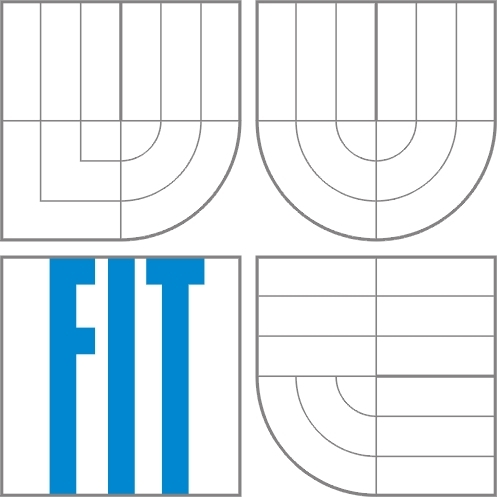
\includegraphics[height=7cm]{logo.jpg}
\end{figure}

\begin{center}
\bigskip
\huge
 Teória obvodov 2014/2015 \\
\end{center}

\begin{center}
\large
\today
\end{center}

\vfill

\begin{flushleft}
\large
\begin{tabular}{ll}
Autor:
& Peter Tisovčík, xtisov00@stud.fit.vutbr.cz \\
& Fakulta Informačcních Technologií \\
& Vysoké Učení Technické v Brně \\
\end{tabular}
\end{flushleft}

\newpage
\begin{center}
\emph{Príklad 1, Varianta A}
\end{center}

\bigskip
Stanovte napätie
$U_{R7}$ a prúd $I_{R7}$.
Použite metódu postupného zjednodušovania obvodu.
\bigskip

Zadané hodnoty:
\begin{center}
\begin{tabular} {| c | c | c | c | c | c | c | c | c | }
\hline
U[V] & $R_1[\Omega]$ & $R_2[\Omega]$ & $R_3[\Omega]$ & $R_4[\Omega]$ & $R_5[\Omega]$ & $R_6[\Omega]$ & $R_7[\Omega]$ & $R_8[\Omega]$\\ \hline
80 & 350 & 650 & 410 & 130 & 360 & 750 & 310 & 190 \\ \hline
\end{tabular}
\end{center}


\begin{figure}[!htb]
\centering
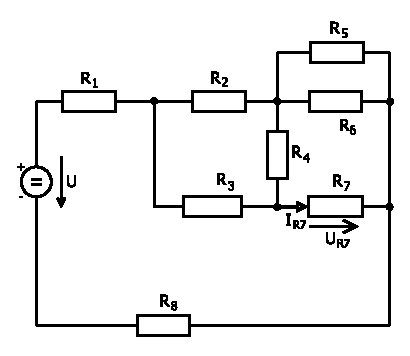
\includegraphics[scale=1.5]{p1/p0.eps}
\caption{Zadanie príkladu číslo 1.}
\end{figure}


1. Paralelné spočítanie odporov  $R_5$ a  $R_6$.
\begin{figure}[!htb]
\centering
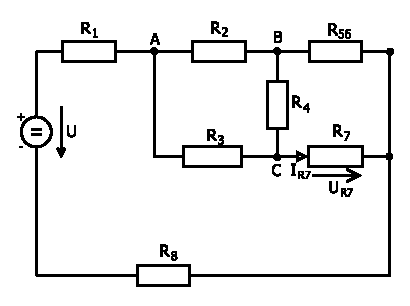
\includegraphics[scale=1.5]{p1/p2.eps}
\caption{Postupné zjednodušovanie obvodu - $R_{56}$}
\end{figure}

\begin{equation}
R_{56} = \frac{R_5 * R_6}{ R_5 + R_6} = \frac{360\Omega*750\Omega}{360\Omega+750\Omega} = 243,2432\Omega
\end{equation}

\newpage
2. Obvod transfigurujeme na hviezdu.
\begin{figure}[!htb]
\centering
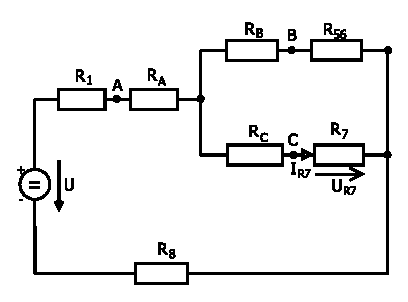
\includegraphics[scale=1.5]{p1/p3.eps}
\caption{Obvod transfigurovaný na hviezdu}
\end{figure}

\begin{equation}
R_A = \frac{R_2 * R_3}{ R_2 + R_3 + R_4} = \frac{650\Omega*410\Omega}{650\Omega+410\Omega+130\Omega} = 223,9496\Omega
\end{equation}

\begin{equation}
R_B = \frac{R_2 * R_4}{ R_2 + R_3 + R_4} = \frac{650\Omega*130\Omega}{650\Omega+410\Omega+130\Omega} = 71,0084\Omega
\end{equation}

\begin{equation}
R_C = \frac{R_4 * R_3}{ R_2 + R_3 + R_4} = \frac{130\Omega*410\Omega}{650\Omega+410\Omega+130\Omega} = 44,7899\Omega
\end{equation}
 \bigskip

3. Sériovo spočítame odpory $R_A$ a $R_1$, $R_B$ a  $R_{56}$, $R_C$ a  $R_7$.
\begin{figure}[!htb]
\centering
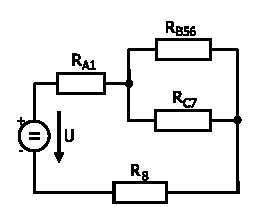
\includegraphics[scale=1.5]{p1/p4.eps}
\caption{Sériové spočítanie odporov}
\end{figure}

\begin{equation}
R_{A1} = R_1 + R_A =350\Omega + 223,9496\Omega = 573,9496\Omega
\end{equation}

\begin{equation}
R_{B56} = R_B + R_{56} =71,0084\Omega + 243,2432\Omega = 314,2516\Omega
\end{equation}

\begin{equation}
R_{C7} = R_C + R_7 =44,7899\Omega +310\Omega = 354,7599\Omega
\end{equation}

\newpage
4. Paralelne vypočítame odpor $R_{B56C7}$.
\begin{figure}[!htb]
\centering
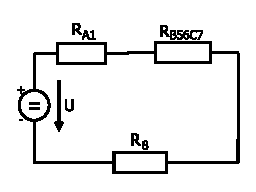
\includegraphics[scale=1.5]{p1/p5.eps}
\caption{Paralelné vypočítanie odporu}
\end{figure}

\begin{equation}
R_{B56C7} = \frac{R_{B56} * R_{C7}}{ R_{B56} + R_{C7}} = \frac{314,2516\Omega*354,7899\Omega}{314,2516\Omega+354,7899\Omega} = 166,6463\Omega
\end{equation}

\bigskip
5. Sériovo spočítame odpory $R_{A1}$, $R_{B56C7}$, $R_{B8}$ a dostaneme $R_{EKV}$.
\begin{figure}[!htb]
\centering
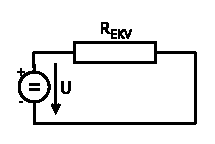
\includegraphics[scale=1.5]{p1/p6.eps}
\caption{Výsledný odpor $R_{EKV}$}
\end{figure}

\begin{equation}
R_{EKV} = R_{A1} + R_{B56C7} + R_8=573,9496\Omega + 166,6463\Omega + 190\Omega = 930,5959\Omega
\end{equation}

\bigskip
6. Výpočet celkového prúdu v obvode na základe vypočítaného odporu $R_{EKV}$.
\begin{equation}
I = \frac{U}{R_{EKV}} = \frac{80V}{930,5959\Omega} = 0,086A
\end{equation}

\bigskip
7. Výpočet prúdu $I_{R7}$ a napätia $U_{R7}$.

\begin{equation}
U_{B56C7} = R_{B56C7} * I = 166.6463\Omega * 0,086A = 14,33V
\end{equation}

\begin{equation}
I_{R7} = I_{C7} = \frac{U_{B56C7}}{R_{C7}} = \frac{14,3316V}{354,7899\Omega} = 0,0404A
\end{equation}

\begin{equation}
U_{R7} = R_7 * I_{R7} = 310\Omega * 0,0404A = 12,524V
\end{equation}



\newpage
\begin{center}
\emph{Príklad 2, Varianta G}
\end{center}

\bigskip
Stanovte napätie
$U_{R3}$ a prúd $I_{R3}$.
Použite metódu Theveninovej vety.
\bigskip

Zadané hodnoty:
\begin{center}
\begin{tabular} {| c | c | c | c | c | c | c | }
\hline
U[V] & $R_1[\Omega]$ & $R_2[\Omega]$ & $R_3[\Omega]$ & $R_4[\Omega]$ & $R_5[\Omega]$ & $R_6[\Omega]$ \\ \hline
180 & 315 & 615 & 180 & 460 & 300 & 270  \\ \hline
\end{tabular}
\end{center}

\begin{figure}[!htb]
\centering
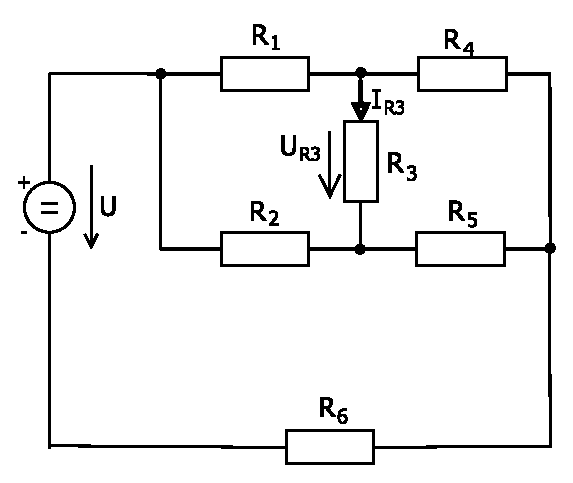
\includegraphics[scale=1.5]{p2/p0.eps}
\caption{Zadanie príkladu číslo 2}
\end{figure}

\newpage
1. Odpor $R_3$ sa vynechá a obvod prekreslíme.
\begin{figure}[!htb]
\centering
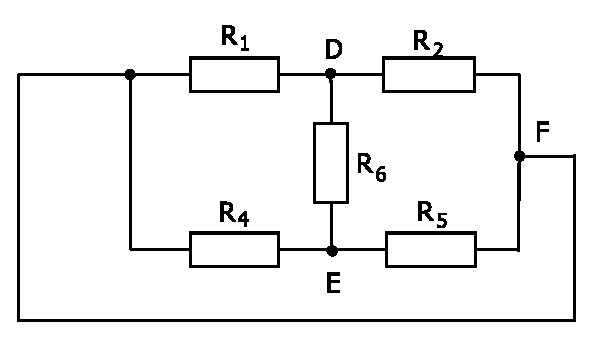
\includegraphics[scale=1.5]{p2/p1.eps}
\caption{Prekreslenie obvodu.}
\end{figure}

\bigskip
2. Obvod transfigurujeme na hviezdu.
\begin{figure}[!htb]
\centering
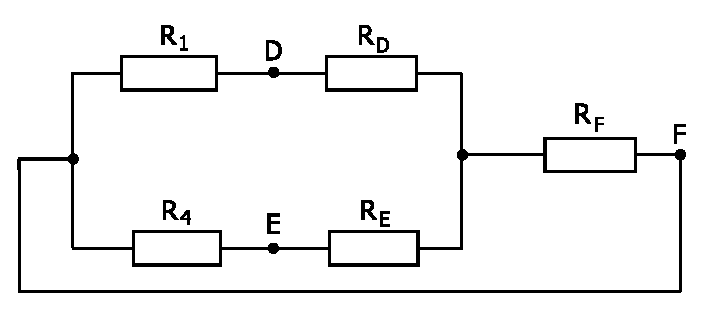
\includegraphics[scale=1.5]{p2/p2.eps}
\caption{Obvod transfigurovaný na hviezdu}
\end{figure}

\begin{equation}
R_D = \frac{R_6 * R_2}{R_2 + R_5 + R_6}
\end{equation}

\begin{equation}
R_E = \frac{R_6 * R_5}{R_2 + R_5 + R_6}
\end{equation}

\begin{equation}
R_F = \frac{R_2 * R_5}{R_2 + R_5 + R_6}
\end{equation}

\newpage
3. Sériovo spočítame odpory $R_1$, $R_D$ a $R_4$, $R_E$.
\begin{figure}[!htb]
\centering
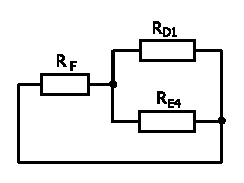
\includegraphics[scale=1.5]{p2/p3.eps}
\caption{Sériovo spočítanie odporov}
\end{figure}


\begin{equation}
R_{D1} = R_D + R_1 = \frac{R_6 * R_2}{R_2 + R_5 + R_6} + R_1
\end{equation}

\begin{equation}
R_{E4} = R_E + R_4 = \frac{R_6 * R_5}{R_2 + R_5 + R_6} + R_4
\end{equation}

\bigskip
4. Výpočet $R_i$.
\begin{figure}[!htb]
\centering
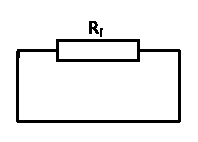
\includegraphics[scale=1.5]{p2/p4.eps}
\caption{Hľadaný odpor $R_i$}
\end{figure}


\begin{equation}
R_i = R_F + \frac {R_{D1} * R_{E4}}{R_{D1} + R_{E4}} = \frac{R_2 * R_5}{R_2 + R_5 + R_6} +
\frac{(\dfrac{R_6 * R_2}{R_2 + R_5 + R_6} + R_1) * (\dfrac{R_6 * R_5}{R_2 + R_5 + R_6} + R_4)}{\dfrac{R_6 * R_2}{R_2 + R_5 + R_6} + R_1 + \dfrac{R_6 * R_5}{R_2 + R_5 + R_6} + R_4} =
\end{equation}

\begin{equation}
= \frac{615\Omega * 300\Omega}{615\Omega + 300\Omega + 270\Omega} +
\frac{(\dfrac{270\Omega * 615\Omega}{615\Omega + 300\Omega + 270\Omega} + 315\Omega) * (\dfrac{270\Omega * 300\Omega}{615\Omega + 300\Omega + 270\Omega} + 460\Omega)}{\dfrac{270\Omega * 615\Omega}{615\Omega + 300\Omega + 270\Omega} + 315\Omega + \dfrac{270\Omega * 300\Omega}{615\Omega + 300\Omega + 270\Omega} + 460\Omega}
\end{equation}

\begin{equation}
= 400,2034\Omega
\end{equation}

\newpage
5. Hodnotu napätia $U_i$ je hodnota medzi uzlami A a B.
\begin{figure}[!htb]
\centering
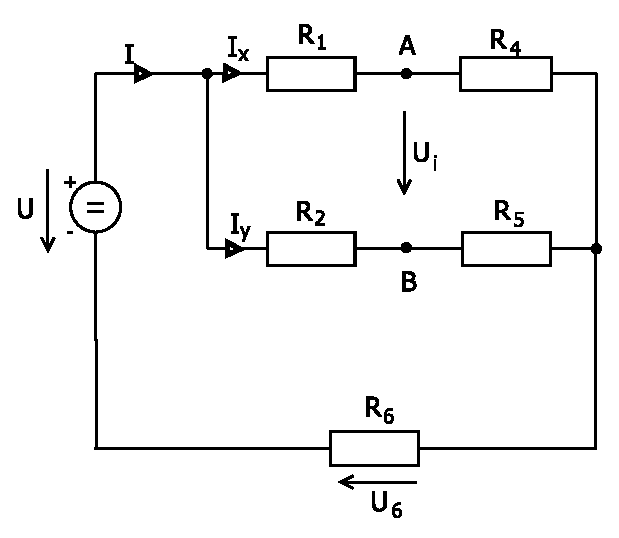
\includegraphics[scale=1.2]{p2/p5.eps}
\caption{Prekreslenie obvodu na výpočet $U_i$}
\end{figure}

6. Výpočet celkového I v obvode pomocou $R_{EKV}$ a výpoočet napätia $U_6$ na odpore $R_6$.

\begin{equation}
R_{EKV} = \frac{(R_1 + R_4) * (R_2 + R_5)}{R_1 + R_4 + R_2 + R_5} + R_6
\end{equation}

\begin{equation}
I = \frac{U}{\dfrac{(R_1 + R_4) * (R_2 + R_5)}{R_1 + R_4 + R_2 + R_5} + R_6} =
\frac{180V}{\dfrac{(315\Omega + 460\Omega) * (615\Omega + 300\Omega)}{315\Omega + 460\Omega + 615\Omega + 300\Omega} +270\Omega} = 0,2610A
\end{equation}

\begin{equation}
U_6 = R_6 * I = 270\Omega * 0,2610A = 70,47V
\end{equation}

\bigskip
7. Zostavenie rovnice pre výpočet prúdov $I_x$ a $I_y$.
\begin{equation}
I_x * R_1 + I_x * R_4 U_6 - U = 0 \Rightarrow I_x = \frac{U - U_6}{R_1 + R_4}
\end{equation}
\begin{equation}
I_y * R_2 + I_y * R_5 U_6 - U = 0 \Rightarrow I_y = \frac{U - U_6}{R_2 + R_5}
\end{equation}

\newpage
8. Výpočet napätia $U_i$
\begin{figure}[!htb]
\centering
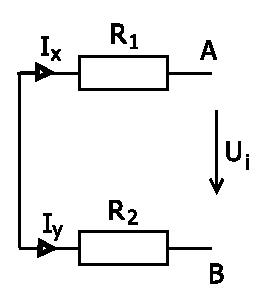
\includegraphics[scale=1.1]{p2/p6.eps}
\caption{Obvod na výpočet $U_i$}
\end{figure}


\begin{equation}
I_x * R_1 + U_ i  - I_y * R_2 = 0  \Rightarrow U_i = I_y * R_2 - I_x * R_1
\end{equation}

\begin{equation}
U_i = \frac{U - U_6}{R_2 + R_5} * R2 - \frac{U - U_6}{R_1 + R_4} * R_1 = \frac{180V - 70,47V}{615\Omega + 300\Omega} * 615\Omega - \frac{180V - 70,47V}{315\Omega + 460\Omega} * 315\Omega = 29,099V
\end{equation}

\bigskip
9. Výpočet hľadaného prúdu $I_{R3}$ a hľadaného napätia $U_{R3}$.
\begin{equation}
I_{R3} = \frac{U_i}{R_i + R_3} = \frac{29,099V}{400,2034\Omega + 180\Omega} = 0,0502A
\end{equation}

\begin{equation}
U_{R3} = R_3 * I_{R3} = R_3 * \frac{U_i}{R_i + R_3} = 180\Omega * \frac{29,099V}{400,2034\Omega + 180\Omega} = 9,0276V
\end{equation}


\newpage
\begin{center}
\emph{Príklad 3, Varianta A}
\end{center}

\bigskip
Stanovte napätie $U_{R5}$ a prúd $I_{R5}$.
Použite metódu uzlových napätí ($U_A$, $U_B$, $U_C$).
\bigskip

Zadané hodnoty:
\begin{center}
\begin{tabular} {| c | c | c | c | c | c | c | c | c | }
\hline
$U_1[V]$ & $U_2[V]$ & I[A] & $R_1[\Omega]$ & $R_2[\Omega]$ & $R_3[\Omega]$ & $R_4[\Omega]$ & $R_5[\Omega]$ & $R_6[\Omega]$ \\ \hline
120 & 90 & 0,7 & 530 & 490 & 650 & 390 & 320 & 120\\ \hline
\end{tabular}
\end{center}

\begin{figure}[!htb]
\centering
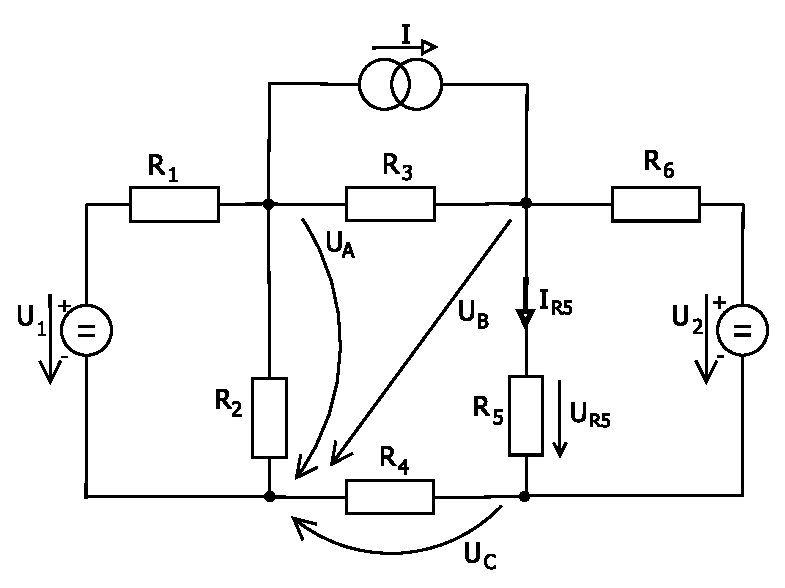
\includegraphics[scale=1.2]{p3/p0.eps}
\caption{Zadanie príkladu číslo 3}
\end{figure}


\newpage
1. Doplnenie označenie uzlov(A, B, C) a smer prúdov($I_{R1}$, $I_{R2}$, $I_{R3}$, $I_{R4}$, $I_{R6}$).
\begin{figure}[!htb]
\centering
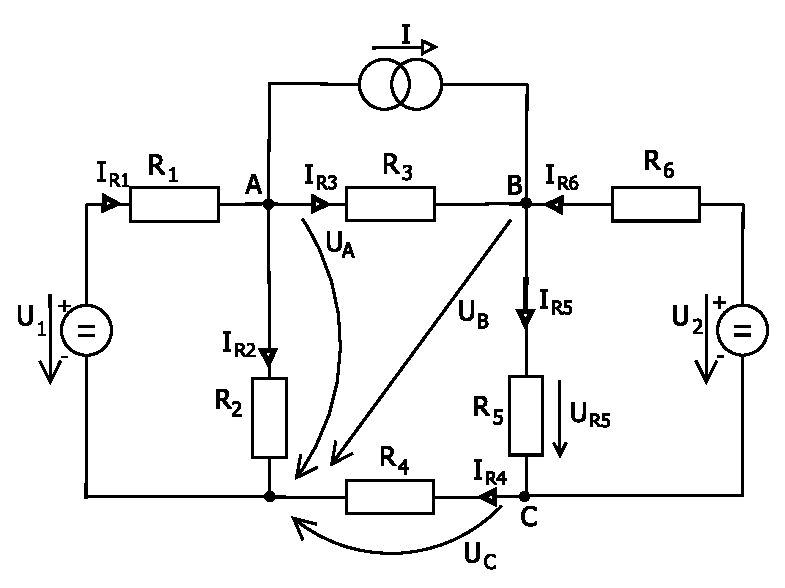
\includegraphics[scale=1.0]{p3/p1.eps}
\caption{Označenie prúdov a uzlov v obvode}
\end{figure}

2. Vyjadrenie rovníc pre uzly A, B, C.
\begin{equation}
A: I_{R1} - I - I_{R3} - I_{R2} = 0
\end{equation}

\begin{equation}
B: I + I_{R3} - I_{R5} + I_{R6} = 0
\end{equation}

\begin{equation}
C: I_{R5} - I_{R6} - I_{R4} = 0
\end{equation}

\bigskip
3. Vyjadrenie jednotlivých prúdov.
\begin{equation}
I_{R1} * R_1 + U_A - U_1 = 0 \Rightarrow I_{R1} = \frac{U_1 - U_A}{R_1}
\end{equation}

\begin{equation}
I_{R2} * R_2 - U_A = 0 \Rightarrow I_{R2} = \frac{U_A}{R_2}
\end{equation}

\begin{equation}
I_{R3} * R_3 + U_B - U_A = 0 \Rightarrow I_{R3} = \frac{U_A - U_B}{R_3}
\end{equation}

\begin{equation}
I_{R4} * R_4 - U_C = 0 \Rightarrow I_{R4} = \frac{U_C}{R_4}
\end{equation}

\begin{equation}
I_{R5} * R_5 + U_C - U_B = 0 \Rightarrow I_{R5} = \frac{U_B - U_C}{R_5}
\end{equation}

\begin{equation}
I_{R6} * R_6 + U_B - U_C - U_2 = 0 \Rightarrow I_{R6} = \frac{U_2 + U_C - U_B}{R_6}
\end{equation}


\newpage
4. Dosadenie prúdov do rovnice pre jednotlivé uzly.
\begin{equation}
A: \frac{U_1 - U_A}{R_1} - I - \frac{U_A - U_B}{R_3} - \frac{U_A}{R_2} = 0 \Rightarrow
I = \frac{U_1 - U_A}{R_1} - \frac{U_A - U_B}{R_3} - \frac{U_A}{R_2}
\end{equation}

\begin{equation}
B: I + \frac{U_A - U_B}{R_3} - \frac{U_B - U_C}{R_5} + \frac{U_2 + U_C - U_B}{R_6} = 0  \Rightarrow
I = \frac{U_B - U_C}{R_5} - \frac{U_A - U_B}{R_3} - \frac{U_2 + U_C - U_B}{R_6}
\end{equation}

\begin{equation}
C: \frac{U_B - U_C}{R_5} - \frac{U_2 + U_C - U_B}{R_6} - \frac{U_C}{R_4} = 0
\end{equation}


\bigskip
\bigskip
5. Dosadenie zadaných hodnôt do rovníc.

\begin{equation}
A: 0,7A = \frac{U_1 - U_A}{530\Omega} - \frac{U_A - U_B}{650\Omega} - \frac{U_A}{490\Omega}
\end{equation}

\begin{equation}
B: 0,7A = \frac{U_B - U_C}{320\Omega} - \frac{U_A - U_B}{650\Omega} - \frac{90V + U_C - U_B}{120\Omega}
\end{equation}

\begin{equation}
C: 0 = \frac{U_B - U_C}{320\Omega} - \frac{90V + U_C - U_B}{120\Omega} - \frac{U_C}{390\Omega}
\end{equation}

\bigskip
\bigskip
6. Po dosadení do matice a výpočte jednotlivých neznámych dostaneme:
\begin{equation}
U_A = -\frac{3836945}{155047} \Rightarrow U_A = -24,747V
\end{equation}

\begin{equation}
U_B = \frac{34095690}{155047} \Rightarrow U_B = 219,9055V
\end{equation}

\begin{equation}
U_C =\frac{19568250}{155047} \Rightarrow U_C = 126,2085V
\end{equation}

\bigskip
\bigskip
7. Výpočet hľadaného napätia $U_{R5}$ a prúdu $I_{R5}$.
\begin{equation}
I_{R5} = \frac{U_B - U_C}{R_5} = \frac{219,9055V - 126,2085V}{320\Omega} = 0,2928A
\end{equation}

\begin{equation}
U_{R5} = I_{R5} * R_5 = 0,2928 * 320\Omega = 93,696V
\end{equation}


\newpage
\begin{center}
\emph{Príklad 4, Varianta A}
\end{center}

\bigskip
Pre napájacie napätie platí: $u = U * \sin (2\pi ft)$. \\
Vo vzťahu pre napätie  $ u_{L_2} = U_{L_2} * \sin (2\pi ft + \varphi_{L_2})$ určite $|U_{L_2}| a \varphi_{L_2}$. Použite metódu zjednodušovania obvodu. \\
\\
Pozn: Pomocný "smer šípky napájacieho zdroja platí pre špecialny časový okamžik $(t = \frac{\pi}{2\omega})$."
\bigskip

Zadané hodnoty:
\begin{center}
\begin{tabular} {|  c | c |  c | c | c | c | c | c | c | }
\hline
U[V] &  $R_1 [\Omega]$  & $R_2 [\Omega]$  &$R_3 [\Omega]$  & $L_1 [mH]$ & $L_2 [mH]$ & $C_1[\mu F]$ & $C_2[\mu F]$  & f [Hz] \\ \hline
45 & 140 & 210 & 340 & 470 & 400 & 210 & 150 & 70\\ \hline
\end{tabular}
\end{center}

\begin{figure}[!htb]
\centering
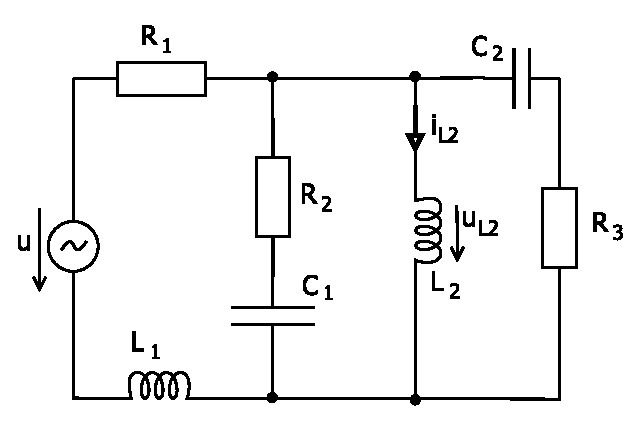
\includegraphics[scale=1.2]{p4/p0.eps}
\caption{Zadanie príkladu číslo 4}
\end{figure}


1. Výpočet jednotlivých impedancií.
\begin{figure}[!htb]
\centering
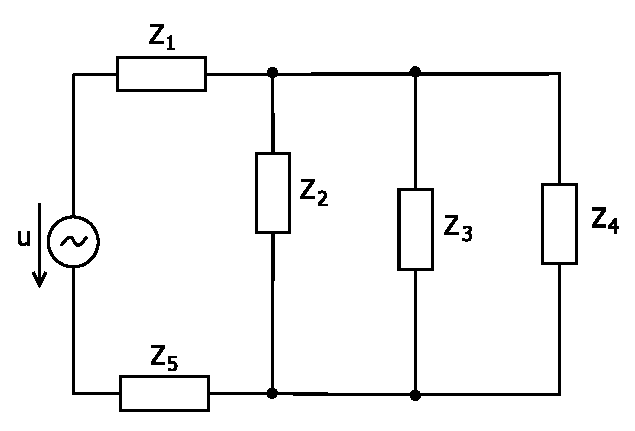
\includegraphics[scale=1.0]{p4/p1.eps}
\caption{Zobrazenie jednotlivých impedancií}
\end{figure}

\newpage
\begin{equation}
\bar{Z_1} = R_1 = 140\Omega
\end{equation}

\begin{equation}
\bar{Z_2} = R_2 - j\frac{1}{\omega C_1} = 210\Omega -j\frac{1}{2\pi * 70Hz * 2,1*10^{-4}} = 210\Omega - j10,8269\Omega
\end{equation}

\begin{equation}
\bar{Z_3} = j\omega L_2 = 2\pi * 70Hz * 0,4H = j175,9292\Omega
\end{equation}

\begin{equation}
\bar{Z_4} = R_3 - j\frac{1}{\omega C_2} = 340\Omega -j\frac{1}{2\pi * 70Hz * 1,5*10^{-4}} = 340\Omega - j15,1576\Omega
\end{equation}

\begin{equation}
\bar{Z_5} = j\omega L_1 = 2\pi * 70Hz * 0,47H = j206,7168\Omega
\end{equation}

\bigskip
\bigskip
2. Zjednodušenie obovodu - paralelné spojenie impedancií $Z_3$, $Z_4$ a $Z_2$.
\begin{figure}[!htb]
\centering
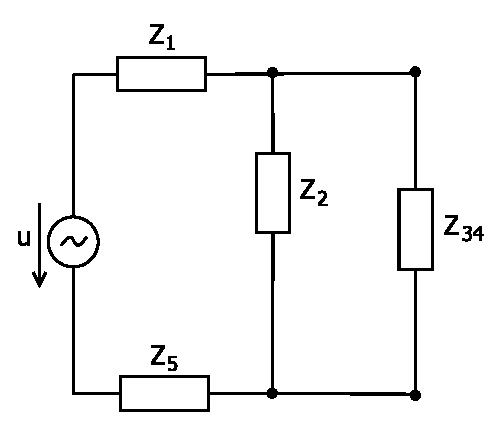
\includegraphics[scale=1.0]{p4/p2.eps}
\caption{Paralelné spojenie impedancií}
\end{figure}

\begin{figure}[!htb]
\centering
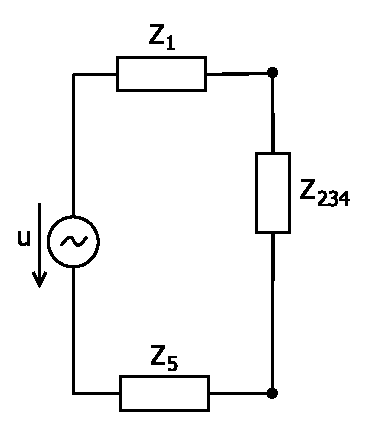
\includegraphics[scale=1.0]{p4/p3.eps}
\caption{Sériové spojenie impedancií}
\end{figure}

\newpage
3. Výpočet celkovej impedancie v obvode.

% 1/x = 1/(210 - 10.8269i) +1/ (175.9292i) +1/ (340 - 15.1576i)
\begin{equation}
\frac{1}{\bar{Z}_{234}} = \frac{1}{\bar{Z_2}} + \frac{1}{\bar{Z_3}} + \frac{1}{\bar{Z_4}} = (88,0937 + 60,8534j)\Omega
\end{equation}

%Celkove
%140 + 88.0937 + 60.8534j + 206.7168i
\begin{equation}
\bar{Z} = \bar{Z}_1 + \bar{Z}_{234} + \bar{Z}_5 = (228,0937 + 267,5702j)\Omega
\end{equation}

\bigskip
4. Výpočet celkového prúdu v obvode.
% 45/(140.0077 + 206.7115i)
\begin{equation}
I = \frac{U}{\bar{Z}} = \frac{45V}{(228,0937 + 267,5702j)\Omega} = (0,0830 -0,0974j)A
\end{equation}

\bigskip
% (88.0937 + 60.8534j) * (0.0830 -0.0974j)
5. Výpočet napätia $U_{234}$, ktoré sa nachádza na impedancií $\bar{Z_2},  \bar{Z_3}, \bar{Z_4}$
\begin{equation}
U_{234} = Z_{234} * I = (88,0937 + 60,8534j)\Omega * (0,0830 -0,0974j)A = (13,2389 - 3,5295j)V
\end{equation}

%sqrt((13.2389)^2 + (-3.5295)^2)
\bigskip
6. Výpočet $\vert U_{L2}\vert$.
\begin{equation}
\vert U_{L2}\vert = \sqrt{Re^2 + Im^2} = \sqrt{(13,2389)^2 + (-3,5295)^2} = 13.7013V
\end{equation}

\bigskip
7. Fázový posun $\varphi _{L2}$.
\begin{equation}
tg \varphi _{L2} = \frac{Im}{Re}
\end{equation}

% arctg(3.5295/13.2389)
\begin{equation}
tg \varphi _{L2} = \frac{-3.5295}{13.2389} = -14,9279^{\circ}
\end{equation}


\newpage
\begin{center}
\emph{Príklad 5, Varianta G}
\end{center}

\bigskip
Pre napájacie napätie platí: $u_1 = U_1 * \sin (2\pi ft)$, $u_2 = U_2 * \sin (2\pi ft)$. \\
Vo vzťahu pre napätie  $ u_{C_1} = U_{C_1} * \sin (2\pi ft + \varphi_{C_1})$ určite $|U_{C_1}| a  \varphi_{C_1}$. Použite metódu zjednodušovania prúdu. \\
\\
Pozn: Pomocný "smery šípiek napájacích zdrojov platí pre špecialny časový okamžik $(t = \frac{\pi}{2\omega})$."
\bigskip

Zadané hodnoty:
\begin{center}
\begin{tabular} {|  c | c | c |  c | c | c | c | c | c | c | }
\hline
$U_1 [V]$ & $U_2 [V]$ &  $R_1 [\Omega]$  & $R_2 [\Omega]$  &$R_3 [\Omega]$  & $L_1 [mH]$ & $L_2 [mH]$ & $C_1[\mu F]$ & $C_2[\mu F]$  & f [Hz] \\ \hline
55 & 50 & 130 & 125 & 155 & 140 & 60 & 160 & 80 & 60\\ \hline
\end{tabular}
\end{center}

\begin{figure}[!htb]
\centering
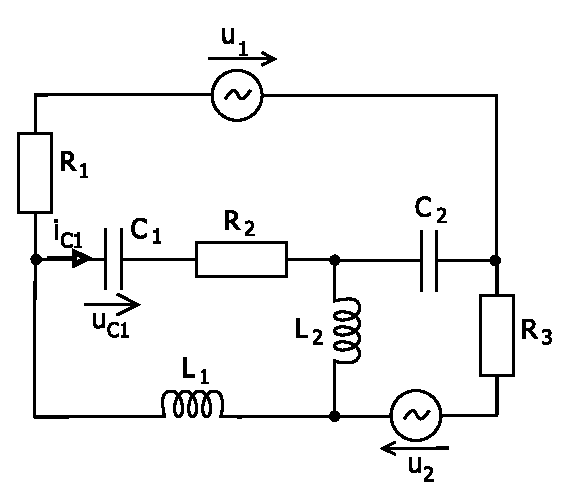
\includegraphics[scale=1.2]{p5/p0.eps}
\caption{Zadanie príkladu číslo 5}
\end{figure}


\newpage
1. Zostavenie jednotlivých rovníc pre jednotlivé slučky a výpočet jednotlivých impedancií.
\begin{figure}[!htb]
\centering
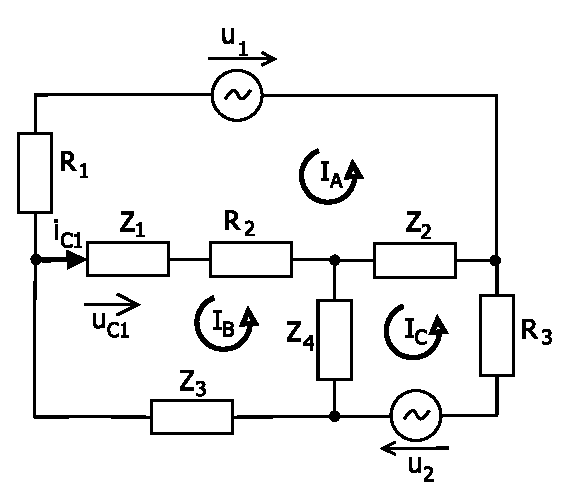
\includegraphics[scale=1.0]{p5/p1.eps}
\caption{Zobrazenie jednotlivých slučiek a impedancií}
\end{figure}


\begin{equation}
Z_1  = \frac{1}{j\omega C_1}  = \frac{1}{j*2*\pi * 60Hz * 1,6*10^{-4}F} = -j16,5786\Omega
\end{equation}

\begin{equation}
Z_2  = \frac{1}{j\omega C_2}  = \frac{1}{j*2*\pi * 60Hz * 0,8*10^{-4}F} = -j33,1573\Omega
\end{equation}

\begin{equation}
Z_3  = j\omega L_1 = j*2*\pi * 60Hz * 0,14H = j52,7788\Omega
\end{equation}

\begin{equation}
Z_4  = j\omega L_2 = j*2*\pi * 60Hz * 0,06H = j22,6195\Omega
\end{equation}

\bigskip
2. Rovnice pre jednotlivé slučkové prúdy.
\begin{equation}
I_A: u_1 * I_A + Z_2 * (I_A - I_C) + R_2 * (I_A - I_B) + Z_1 * (I_A - I_B) + R_1 * I_A = 0
\end{equation}

\begin{equation}
I_B: Z_1 * (I_B - I_A) + R_2 * (I_B - I_A) + Z_4 * (I_B - I_C) + Z_3 * I_B = 0
\end{equation}

\begin{equation}
I_C: Z_2 * (I_C - I_A) + R_3 * I_C + u_2 + Z_4 * (I_C - I_B) = 0
\end{equation}

\bigskip
3. Dosadenie hodnôt do rovníc.
\begin{equation}
I_A: 55 * I_A -j33,1573 * (I_A - I_C) + 125 * (I_A - I_B) -j16,5786 * (I_A - I_B) + 130 * I_A = 0
\end{equation}

\begin{equation}
I_B: -j16,5786 * (I_B - I_A) + 125 * (I_B - I_A) + j22,6195 * (I_B - I_C) + j52,7788 * I_B = 0
\end{equation}

\begin{equation}
I_C: -j33,1573 * (I_C - I_A) + 155 * I_C + 50 + j22,6195 * (I_C - I_B) = 0
\end{equation}

\newpage
4. Úprava rovníc.
\begin{equation}
55 + (255 -49.7359j)I_A + (-125 + 16.5786j)I_B + (33.1573j)I_C = 0
\end{equation}

\begin{equation}
(125 + 58.8197j)I_B+ (-125+ 16.5786j)I_A +(- 22.6195j)I_C = 0
\end{equation}

\begin{equation}
(155 - 10.5378j)I_C + (33.1573j)I_A + (-22.6195j)I_B + 50 = 0
\end{equation}

\bigskip
5. Výpočet jednotlivých prúdov.
\begin{equation}
I_A = (-0,3376 + 0,0822j)A
\end{equation}

\begin{equation}
I_B = (-0,2438 + 0,1816j)A
\end{equation}

\begin{equation}
I_C = (-0,3324 + 0,0140j)A
\end{equation}

\bigskip
6. Výpočet prúdu $I_{C1}$.
\begin{equation}
I_{C} = I_B - I_A = (-0,2438 + 0,1816j)A - (-0,3376 + 0,0822j)A = (0,0938 + 0,0994j)A
\end{equation}

\bigskip
7. Výpočet napätia $U_{C1}$.
\begin{equation}
U_{C1} = Z_1 * I_{C1} = -j16,5786\Omega * (0,0938 + 0,0994j)A = (1,6479 - 1,5551j)V
\end{equation}

\bigskip
8. Výpočet $|U_{C1}|$.
\begin{equation}
\vert U_{C1}\vert = \sqrt{Re^2 + Im^2} = \sqrt{(1,6479)^2 + (-1,5551)^2} = 2,2658V
\end{equation}

\bigskip
9. Fázový posun $\varphi _{C1}$.
\begin{equation}
tg \varphi _{C1} = \frac{Im}{Re}
\end{equation}

% arctg(-1.5551/1.6479)
\begin{equation}
tg \varphi _{C1} = \frac{1,6479}{-1,5551} = -43,3404^{\circ}
\end{equation}

\begin{equation}
180^{\circ} - 43,3404^{\circ} = 136,6596^{\circ}
\end{equation}

\newpage
\begin{center}
\emph{Príklad 6, Varianta A}
\end{center}

\bigskip
Zostavte diferenciálnu rovnicu popisujúcu chovanie obvodu na obŕazku, ďalej ju upravte dosadením hodnôt parametru. Vypočítajte analytickej riešenie
$i_L = f(t)$. Urobte kontrolu výpočtu dosadením do zostavenej diferencialnej rovnice.
\bigskip

Zadané hodnoty:
\begin{center}
\begin{tabular} {|  c | c | c | c |}
\hline
U [V] & L [H] & R  $[\Omega]$ & $i_L (0) [A]$ \\ \hline
20 & 40 & 10 & 9\\ \hline
\end{tabular}
\end{center}

\begin{figure}[!htb]
\centering
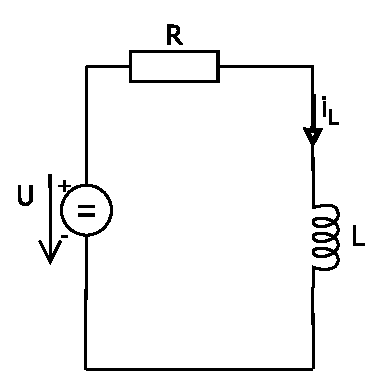
\includegraphics[scale=1.0]{p6/p0.eps}
\caption{Zadanie príkladu číslo 6}
\end{figure}

\bigskip
1. Na vytvorenie diferenciálnej rovnice cievky použijeme nasledujúci axióm.
\begin{equation}
i'_L = \frac{u_L}{L}
\end{equation}

2. Určíme si napätie $u_L$ a dosadíme do rovnice.
\begin{equation}
i_L * R + u_L - U = 0 \Rightarrow u_L = U - i_L * R
\end{equation}

\begin{equation}
L * i'_L =  U - i_L * R \Rightarrow   U = L * i'_L + i_L * R
\end{equation}

\bigskip
3. Vyjadrenie $\lambda$ z rovnice.
\begin{equation}
L\lambda + R = 0 \Rightarrow 40\lambda + 10 = 0 \Rightarrow \lambda = -\frac{1}{4}
\end{equation}

4. Očakávané riešenie.
\begin{equation}
i_L(t) = c(t)*e^{\lambda t} \Rightarrow i_L(t) = c*e^{-\frac{1}{4} t}
\end{equation}

\bigskip
5. Výpočet $i'_L$.
\begin{equation}
i'_L = c'*e^{-\frac{1}{4} t} + (-\frac{1}{4}) * c*e^{-\frac{1}{4} t}
\end{equation}

\newpage
6. Dosadenie do obecného tvaru a zderivovanie.
\begin{equation}
40*(c'*e^{-\frac{1}{4} t} + (-\frac{1}{4}) * c*e^{-\frac{1}{4} t}) + 10*(c*e^{-\frac{1}{4} t}) = 20
\end{equation}

\begin{equation}
40c'*e^{-\frac{1}{4} t} -10 * c*e^{-\frac{1}{4} t}) + 10*c*e^{-\frac{1}{4} t} = 20
\end{equation}

\begin{equation}
40c'*e^{-\frac{1}{4} t} = 20
\end{equation}

7. Vyjadrenie c'.
\begin{equation}
40c'*e^{-\frac{1}{4} t} = 20 \Rightarrow c' = \frac{20}{40*e^{-\frac{1}{4} t}} \Rightarrow c' = \frac{1}{2}*e^{\frac{1}{4} t}
\end{equation}

\bigskip
8. Odstránenie derivácie - zintegrovanie.
\begin{equation}
c(t) + K_1 = \frac{4}{1} * \frac{1}{2}*e^{\frac{1}{4} t} + K_2 \Rightarrow c(t) = 2*e^{\frac{1}{4} t} + K
\end{equation}

9. Dosadenie do očakávaného riešenia, výpočet konštanty K.
\begin{equation}
i_L(0) = c(0) * e^{\lambda 0}
\end{equation}

\begin{equation}
9 =  2*e^{\frac{1}{4} 0} + K*e^{-\frac{1}{4} 0} \Rightarrow K = 7
\end{equation}

10. Dosadenie konštanty do riešenia.
\begin{equation}
i_L(t) = (2*e^{\frac{1}{4} t} + 7)*e^{-\frac{1}{4} t}
\end{equation}

\begin{equation}
i_L(t) = 2*e^{\frac{1}{4} t} * e^{-\frac{1}{4} t}  + 7 * e^{-\frac{1}{4} t}
\end{equation}

\begin{equation}
i_L(t) = 2 + 7 * e^{-\frac{1}{4} t}
\end{equation}

\bigskip
11. Skúška.
\begin{equation}
i =  2 + 7 * e^{-\frac{1}{4} t}
\end{equation}

\begin{equation}
i' =  -\frac{7}{4} * e^{-\frac{1}{4} t}
\end{equation}

\begin{equation}
40*(-\frac{7}{4} * e^{-\frac{1}{4} t} ) + 10*(2 + 7 * e^{-\frac{1}{4} t} ) = 20
\end{equation}

\begin{equation}
-70 * e^{-\frac{1}{4} t} + 20 + 70 * e^{-\frac{1}{4} t}  = 20
\end{equation}

\begin{equation}
20 = 20
\end{equation}
\newpage
\begin{center}
\textbf{Tabuľka výsledkov}
\end{center}

\begin{center}
\begin{tabular}{|c|c|l|}
\hline
Príklad č.  & Skupina & Výsledok                            \\ \hline
1 & A & $U_{R7}$ = 12,524V  \hspace{7mm} $I_{R7}$ = 0,404A \\ \hline
2 & G & $U_{R3}$ = 9,0276V \hspace{7mm}  $I_{R3}$ = 0,502A \\ \hline
3 & A & $U_{R5}$ = 93,696V \hspace{7mm} $I_{R5}$ = 0,2928A \\ \hline
4 & A & $|U_{L2}|$ = 13,7013V  \hspace{3mm} $\varphi_{L2}$ = $ -14,9279^{\circ}$  \\ \hline
5 & G & $|U_{C1}|$ = 2,2658V  \hspace{5mm} $\varphi_{C1}$ = $136,6596^{\circ}$         \\ \hline
6 & A & $i_L(t) = 2 + 7 * e^{-\frac{1}{4} t} $                                  \\ \hline
\end{tabular}
\end{center}


\end{document}
